\section{Atividade 3}

\subsection{Descrição do Modelo e Análise de Sistema}
Nesta atividade, foi desenvolvida a função de transferência para um sistema massa-mola-amortecedor com os seguintes parâmetros específicos para o estudante Guilherme Cagide Fialho:
\begin{itemize}
    \item Massa, \( m = 10 \) kg.
    \item Coeficiente de amortecimento, \( C = 7 \) Ns/m.
    \item Constante da mola, \( K = 5 \) N/m.
\end{itemize}
A função de transferência obtida é:
\[
G(s) = \frac{1}{10s^2 + 7s + 5}
\]

\subsection{Cálculo dos Polos e Parâmetros do Sistema}
Os polos da função de transferência são complexos conjugados e foram calculados como:
\begin{itemize}
    \item Polo 1: \( -0.35 + 0.614j \)
    \item Polo 2: \( -0.35 - 0.614j \)
\end{itemize}

Os parâmetros típicos do sistema de segunda ordem são:
\begin{itemize}
    \item Frequência natural não-amortecida (\( \omega_n \)): \( 0.707 \) rad/s
    \item Coeficiente de amortecimento (\( \zeta \)): \( 0.495 \)
    \item Ganho estático (\( K_p \)): \( 0.2 \)
\end{itemize}

\subsection{Resposta ao Impulso}
A resposta ao impulso do sistema foi simulada e é mostrada na figura abaixo:
\begin{figure}[H]
    \centering
    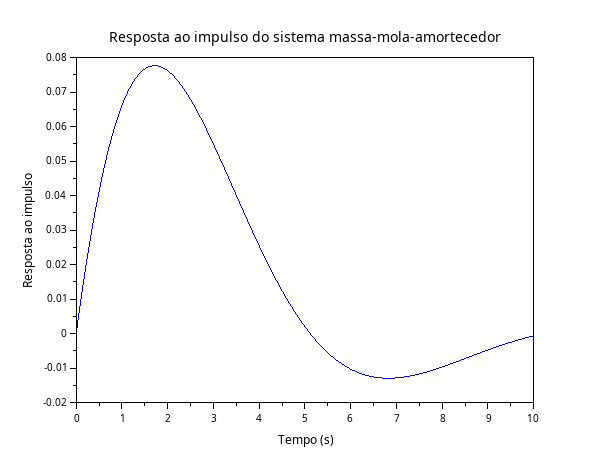
\includegraphics[width=0.8\textwidth]{3-atividade/assets/resposta-ao-impulso.png}
    \caption{Resposta ao impulso do sistema massa-mola-amortecedor}
\end{figure}

\subsection{Discussão}
A análise dos polos mostra que o sistema é subamortecido, o que é corroborado pelo coeficiente de amortecimento menor que 1. A resposta ao impulso ilustra um comportamento oscilatório decaído, típico de sistemas subamortecidos, onde as oscilações diminuem gradualmente até a estabilização. O ganho estático (\( K_p \)) indica a resposta do sistema a uma entrada de degrau unitário em regime permanente.

\subsection{Conclusões}
A simulação e os cálculos realizados fornecem uma visão detalhada da dinâmica do sistema, evidenciando como os parâmetros de massa, amortecimento e rigidez influenciam o comportamento do sistema. Esta análise é essencial para o entendimento e design de sistemas de controle que possam efetivamente gerenciar tais dinâmicas.
